\documentclass[12pt, twoside]{article}
\usepackage[letterpaper, margin=1in, headsep=0.5in]{geometry}
\usepackage[english]{babel}
\usepackage[utf8]{inputenc}
\usepackage{amsmath}
\usepackage{amsfonts}
\usepackage{amssymb}
\usepackage{tikz}
\usetikzlibrary{quotes, angles}
\usepackage{graphicx}
\usepackage{enumitem}
\usepackage{multicol}

\newif\ifmeta
\metatrue %print standards and topics tags

\title{Regents Geometry}
\author{Chris Huson}
\date{September 2020}

\usepackage{fancyhdr}
\pagestyle{fancy}
\fancyhf{}
\renewcommand{\headrulewidth}{0pt} % disable the underline of the header
\raggedbottom


\fancyhead[LE]{\thepage}
\fancyhead[RO]{\thepage \\ Name: \hspace{4cm} \,\\}
\fancyhead[L]{BECA / Dr. Huson / Geometry 06-Analytic-geometry\\* pset ID: 93}

\begin{document}

\subsubsection*{6-8xHW-Trig-intro}
\begin{enumerate}
\item Express the result to \emph{the nearest hundredth}.  \vspace{0.5cm}
    \begin{multicols}{2}
      \begin{enumerate}
        \item $\sin 32^\circ = $ \vspace{0.5cm}
        \item $\cos 29^\circ =$
        \item $\cos 58^\circ = $ \vspace{0.5cm}
        \item $\sin 61^\circ =$
      \end{enumerate}
    \end{multicols}

\item $\triangle ABC$ is shown with $m\angle C=90^\circ$. The lengths of the triangle's sides are $a$, $b$, and $c$. Express each trigonometric ratio as a fraction of two variables. \vspace{1cm}
  \begin{multicols}{2}
      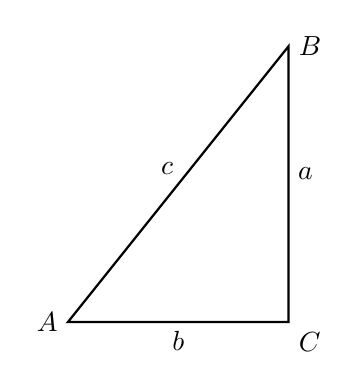
\begin{tikzpicture}[scale=0.7]
        \draw [thick]
        (0,0)node[left]{$A$}--
        (4,0)node[below right]{$C$}--
        (4,5)node[right]{$B$}--cycle;
        \node at (2,0)[below]{$b$};
        \node at (4,2.7)[right]{$a$};
        \node at (1.8,2.5)[above]{$c$};
      \end{tikzpicture}

        \begin{enumerate}
        \item $\sin B =$ \vspace{0.75cm}
        \item $\cos B =$ \vspace{0.75cm}
        \item $\tan B =$ \vspace{0.75cm}
      \end{enumerate}
  \end{multicols}

  
\item Given right $\triangle JKL$ with $\overline{JK} \perp \overline{KL}$, $JL=12.4$, $m\angle J=41^\circ$. Find the length $JK$, \emph{rounded to the nearest hundredth}.
    \begin{center}
      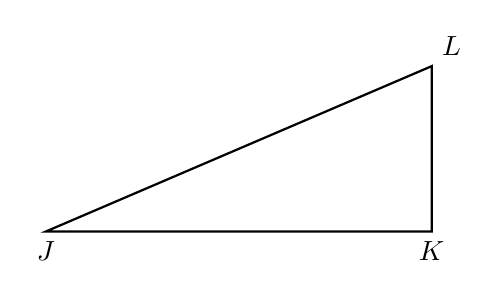
\begin{tikzpicture}[scale=0.7]
        \draw [thick]
        (0,0) node[below]{$J$}--
        (7,0)  node[below]{$K$}--
        (7,3) node[above right]{$L$}--cycle;
      \end{tikzpicture}
    \end{center}

    %\vspace{4cm}

\newpage


\item Spicy: On the set of axes below, graph the quadrilateral $ABCD$ having coordinates $A(-3,-3)$, $B(5,1)$, $C(6,8)$, and $D(-2,4)$.
    \begin{center} %4 quadrant regents grid
    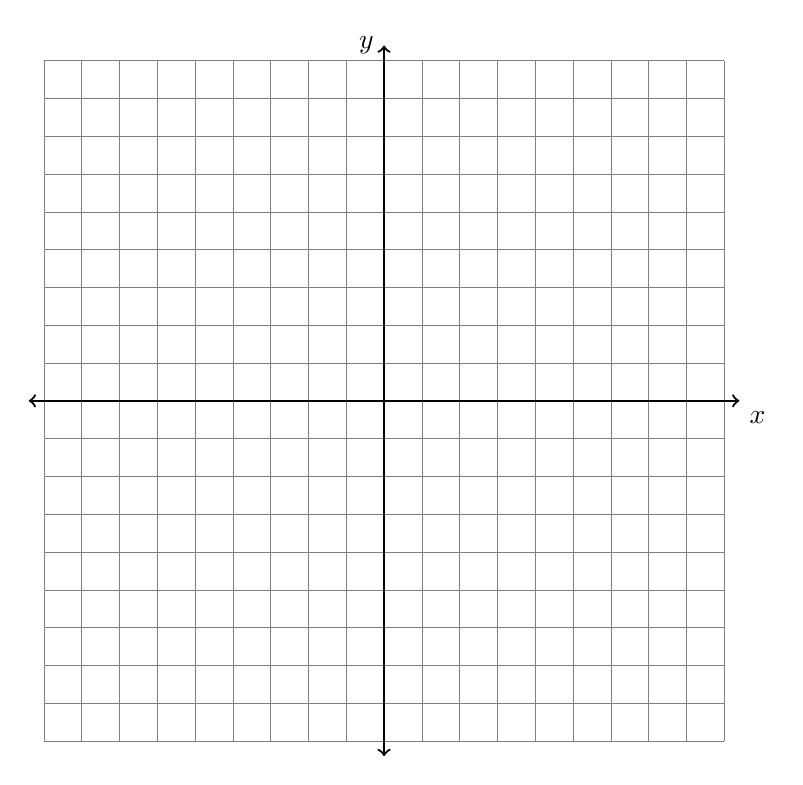
\begin{tikzpicture}[scale=.48]
      \draw [help lines] (-9,-9) grid (9,9);
      \draw [thick, <->] (-9.4,0) -- (9.4,0) node [below right] {$x$};
      \draw [thick, <->] (0,-9.4)--(0,9.4) node [left] {$y$};
      %\draw [thick] (-3,-3) node[below] {$A$}--
      %(5,1) node[right] {$B$}--
      %(6,8) node[left] {$C$}--
      %(-2,4) node[left] {$D$}--cycle;
      %\draw [fill] (5,0) circle [radius=0.1] node[above left] {$P$};
    \end{tikzpicture}
    \end{center}
    Given that $\overline{AD} \perp \overline{BC}$. Use what you know about slope and the definition that a parallelogram is a quadrilateral with two pairs of parallel sides to prove $ABCD$ is a parallelogram. Be sure to state the conclusion in your proof.



\end{enumerate}
\end{document}